\pagestyle{fancy}

\graphicspath{ {Figures/Chapter7_GSI/} }

In June 2022 a dedicated set of measurements were performed in GSI (Darmstadt, Germany) for the commissioning of two SEM grid prototypes. The design and production of the SEM Grids were performed by the company PROACTIVE R$\&$D \parencite[][]{ref:ProactiveRND}. In this chapter, we shall discuss the motivation of the experiment and the experimental details and conditions. This is followed by a summary of the most relevant results. Part of these results have been already presented in LINAC2022 \parencite[][]{ref:Linac2022Thomas} and in IBIC2022 \parencite[][]{ref:Ibic2022Juan}. 

\section{The FAIR project and UNILAC}

The GSI Helmholtz Centre for Heavy Ion Research is a heavy ion research center in Darmstadt, Germany. The main focus of the GSI research program is the basic investigation in the field of nuclear physics and atomic physics \parencite[][]{ref:GSI}. Figure \ref{fig:GSIlayout} shows a schematic representation of the GSI accelerator complex. GSI is unique among research facilities worldwide in that it can generate positively charged ions of many different naturally occurring elements, from protons to uranium. 

\begin{figure}[h]
    \centering
    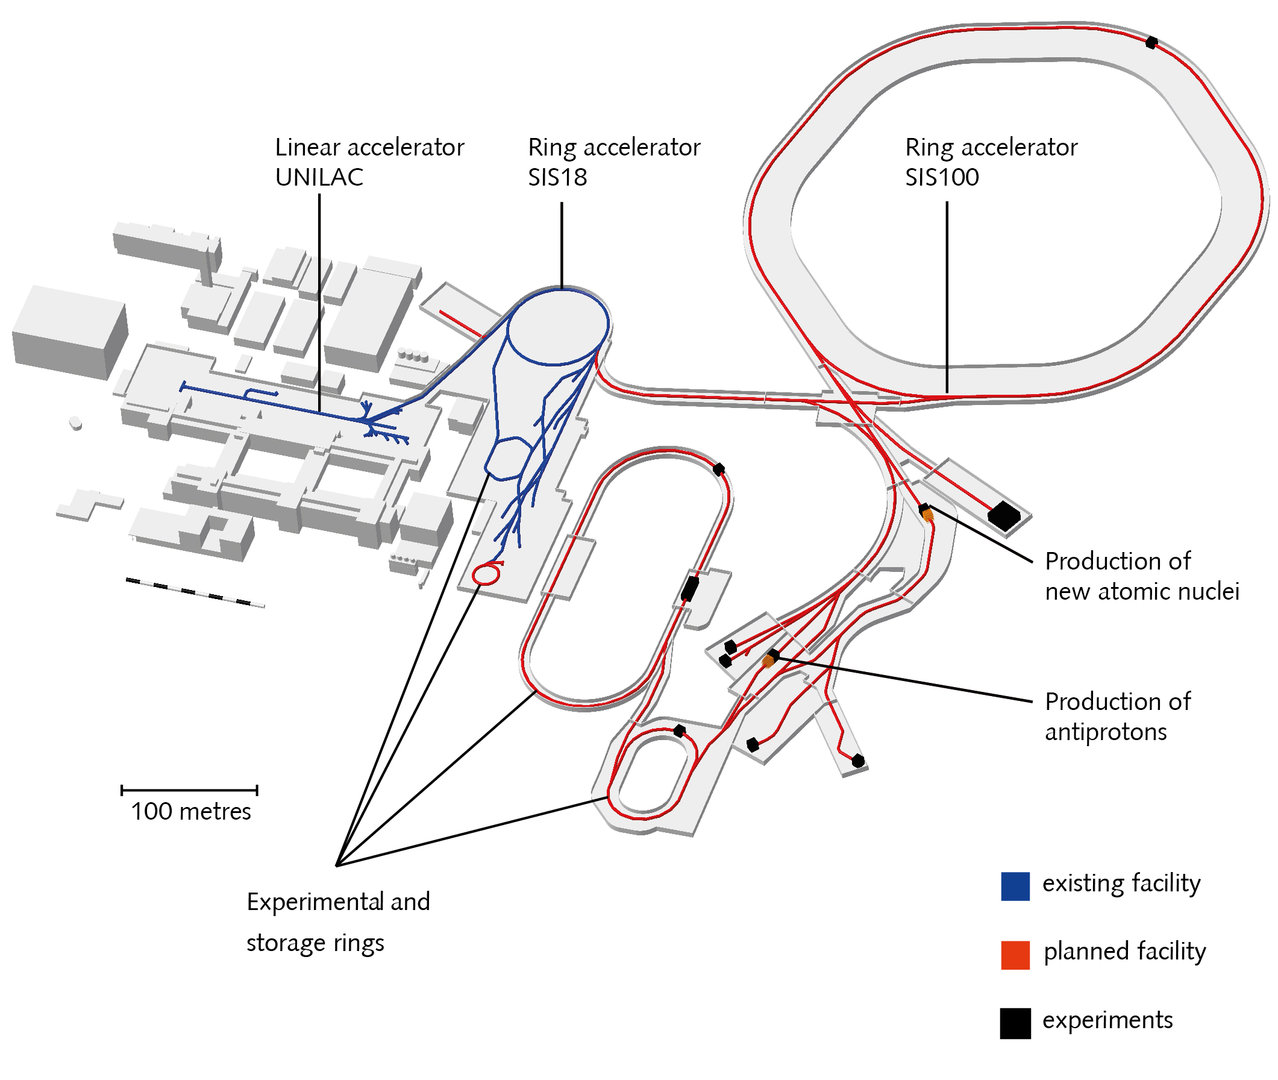
\includegraphics[width=0.66\columnwidth]{GSIFacility/GSIFacility.jpg}
    \caption{Layout of the GSI + FAIR accelerator facility.}
    \label{fig:GSIlayout}
\end{figure}

The process beings at the linear accelerator UNILAC  (The UNIversal Linac ACcelerator), where the different types of ions are produced. Figure \ref{fig:UNILAC} shows a more detailed schematic representation of GSI's UNILAC accelerator. Two of the ion sources are placed at the beginning of the LINAC and one is placed in the middle. After the extraction from the source, the dc-beam is bunched and pre-accelerated by the RFQ, and then accelerated along the Inter-Digital (IH) cavities up to 1.4 MeV/u. 

In some cases, before the next accelerator step, the ions are passed through a gaseous medium to strip them off the outer electrons and thus augment the ion charge state of the beam. The final energy of 11.4 MeV/u is achieved using five Alvarez-Type cavities \parencite[]{ref:AlvarezCavity}. A unique feature of the UNILAC is that some of the Alvarez-Cavities can be operated without acceleration, hence also energies of 3.6, 4.8, 5.9 and 8.6 MeV/u can be provided. 

\begin{figure}[h]
    \centering
    \includegraphics[width=1.0\columnwidth]{UNILACfacility/Unilinac2.png}
    \caption{Schematic representation of UNILAC accelerator.}
    \label{fig:UNILAC}
\end{figure}


After the UNILAC, the beam can be directed to the experimental Hall (EH) or injected to the transfer line (TK), which can provide an additional stripping foil and charge state separation of heavier ions for the future injection to the heavy ion synchrotron SIS18. SIS18 is a versatile synchrotron, with a circumference of 216 m. In SIS18 the ions are accelerated to adjustable energy whose peak value depends on the mass-to-charge ratio of the particle beam. 

To accommodate the demand for higher beam energy and intensity for more advanced physics experiments, the international Facility for Antiproton and Ion Research (FAIR) is currently being constructed at GSI \parencite*[]{ref:FAIR}. FAIR will include three linear accelerators: UNILAC, a superconducting cw-Linac \parencite*[]{ref:cwLinac} and the new proton Linac (pLinac) \parencite[][]{ref:pLinac}. The UNILAC and pLinac will be the main injectors of SIS18, which will in turn be an injector for SIS100, the central accelerator component of FAIR. It is planed for the pLinac to deliver a current up to 70 mA with a macro-pulse length of 35 $\mu s$ (at max. 4 Hz) and a typical bunch length of 100 ps. The design energy is 68 MeV. Special care has to be taken for the design of the diagnostics for this accelerator due to the challenging beam conditions. The overall diagnostics concept and layout of pLinac have been described in various reports, e.g. \parencite[][]{ref:InstruLinac}. 

\section{Motivation and Experimental Conditions}

To measure the transverse beam profile in the future pLinac, the traditional SEM grid design of GSI (64 wires with 2.0 mm spacing ) had to be modified. For that, a new set of grids for the pLinac were designed by PROACTIVE R$\&$D company in collaboration with GSI. To test the two newly designed SEM grid Prototypes two measuring campaigns were performed. In the first campaign, a low-intensity proton beam was used to prove the correct function of the Grid in connection with the POLAND $+$ CSA electronics \parencite[]{ref:ElectronicsSEMgsi}. In the second campaign, which took place in June 2022, a high-intensity Argon beam was used to mimic the pLinac beam conditions. 

\begin{figure}[h]
    \centering
    \includegraphics[width=0.8\columnwidth]{SEMGridProac/SemGridProac.png}
    \caption{SEM grid by PROACTIVE R$\&$D. }
    \label{fig:SEMGridProactive}
\end{figure}

Two SEM grid prototypes were tested. Figure \ref{fig:SEMGridProactive} shows a picture of one of the SEM grids tested during these measurements. Both SEM Grids had 64 wires, with a wire spacing of 0.5 mm.  The active area is 32 x 32 $mm^2$. The only difference between the SEM grid prototypes was the wire material. One grid had 100 $\mu m$ gold-tungsten wires (we will call it Grid1). The other grid had 100 $\mu m$ pure tungsten wires (we will call it Grid2).

Besides the high resolution and compact design, special care was taken for the implementation of the diamond-shaped cleaning electrode. These electrodes are kept to a positive potential to enhance secondary emission and prevent the emitted SE from being captured by neighboring wires. The electric field distribution and the optimal potential required were studied in detail as shown in \parencite*[]{ref:ElectriFieldStudies}. Moreover, a specially designed stretching system is used PROACTIVE grids to keep the wires under tension during irradiation.

\begin{table}[h]
    \centering

    \begin{tabular}{ccccc}
    \hline
    Ion   & \begin{tabular}[c]{@{}c@{}}Energy\\ (MeV/u)\end{tabular} & \begin{tabular}[c]{@{}c@{}}Intensity\\ (mA)\end{tabular} & \begin{tabular}[c]{@{}c@{}}Pulse Length\\ ($\mu s$)\end{tabular} & \begin{tabular}[c]{@{}c@{}}Rep Rate\\ (Hz)\end{tabular} \\ \hline
    $Ar^{10+}$ & 8.6     & 0.04 - 1.5        & 40 - 200       & 1      \\ \hline
    \end{tabular}

    \caption{Summary of beam conditions for measurements.}
    \label{tab:BeamConditions}

\end{table}

The main objective of this second experimental campaign was to check the wire stretching system, the effect of the voltage on the cleaning electrodes and to measure the upper limit of acceptable energy deposition on the detector. In parallel to the measurements, simulations for wire heating were done with the pyTT code, predicting the wire temperature at the various measurements. 

The experiments were performed in the UNILAC Experimental Hall, at the X2 experimental Line. Table \ref{tab:BeamConditions} summarizes the beam conditions used during this experimental campaign. The beam current could be measured using a BCT placed upstream of the SEM grid and a faraday cup placed downstream of the grid. An independent measurement of the beam profile could also be measured by using a GSI SEM grid installed upstream of the beam pipe. The Proactive SEM grid was connected to the POLAND + CSA electronics. The data of the measurements could be visualized in real-time and they were also stored for offline analysis. Data storage of the other devices used during these measurements was not available, those measurements rely on the data taken on the fly. 

\section{Experimental Results}

\subsection{Bias Voltage Studies}

This part of the measurements focused on testing the effects of the voltage on the diamon-shaped cleaning electrodes for different beam conditions. Following the formula introduced in \ref{ch:BeamMatterInter}, one can calculate the expected signal to be generated on the wires. Specifically this would be:
\begin{equation}
    Q\left(\frac{e}{Ar^{10+}}\right) = 18\eta - 8 \mu + 18SEY_{p}\left( 2 - \eta + BS_{p}\right) + 8SEY_{e}\left(2 - \mu + BS_{e}\right)
\end{equation}
The parameters necessary to complete this expression are summarized in table \ref{tab:CurrentParAr10}. Note that in this case, both $\eta$ and $\mu$ are 1.0. This means that both the protons and the electrons of the Argon ion deposit their full charge in the material. The range of argon in Tungsten is 11.8 $\mu m$, which is much smaller than the thickness of the wires (100 $\mu m$). The secondary emission yields and backscattering probabilities given in table \ref{tab:CurrentParAr10} were calculated without considering any electric field. 
\begin{table}[h]
    \centering
    \begin{tabular}{cccccccc}
    \hline
    $\eta$ & $\mu$ & $SEY_p$ & $SEY_e$ & $BS_p$ & $BS_e$ & & Q(e/Ar) \\ \hline
      1.0  &  1.0  &  14.91    &  $8.608\cdot 10^{-6}$   & 0.0    &  0.0 & & 278.38  \\ \hline
    \end{tabular}
    \caption{Summary of parameters necessary for calculating charge generation in a wire(Tungsten, $\phi $ = 100 $\mu m$) by a particle beam ($Ar^{10+}$ ion at 8.6 MeV/uma). These parameters were calculated with Geant4.}
    \label{tab:CurrentParAr10}
\end{table}

\begin{figure}[h]
    \vspace{-0.4cm}
    \centering
    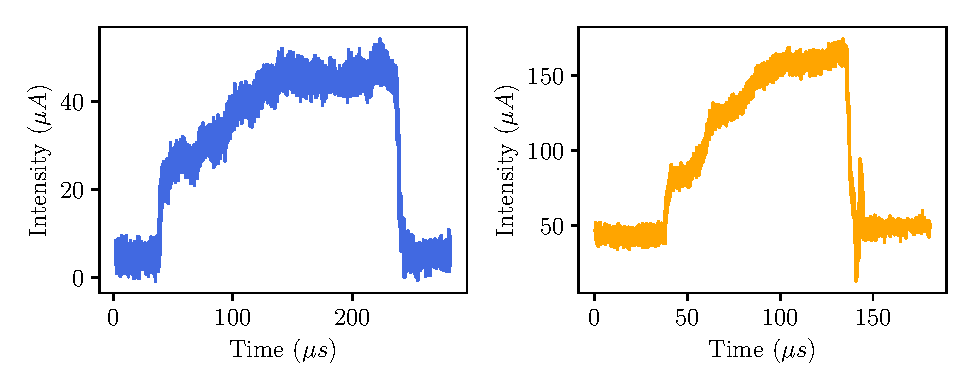
\includegraphics[width=0.95\columnwidth]{BCTSignalExample/BCTSignalExamples.pdf}
    \caption{Intensity as a function of time, measured by the BCT, during one beam pulse. For two different beam conditions, 40 $\mu s$ (left) and 150 $\mu s$ (right).}
    \label{fig:BCTExample}
\end{figure}

The electric field generated by the bias plates slightly affects these parameters. A sufficiently high positive voltage could slightly enhance the SEY. However, it is not straightforward to give a quantitative value of that change \parencite[]{ref:VoltageOnSEY1}  \parencite[]{ref:VoltageOnSEY2}. The applied voltage also helps reduce the SE crosstalk. This means it will prevent SE emitted from one wire to deposit their charge in another wire. A clear positive signal will be generated in the wires due to their interaction with the Argon beam. We expect this signal to be enhanced when a positive bias is applied to the electrodes and to be reduced when a negative bias is applied to them.

A relative error of $10\%$ was considered in all the points. This error is due to fluctuations in the beam intensity during the measurements. The intensity of the beam was not constant along the beam pulse, this can be observed in Figure \ref{fig:BCTExample} where the intensity of the beam measured by the BCT is shown, for two different beam pulse lengths. Moreover, shot-by-shot intensity fluctuations were also observed. 

\begin{figure}[t]
    \centering
    \begin{subfigure}{1.0\columnwidth}
        \centering
        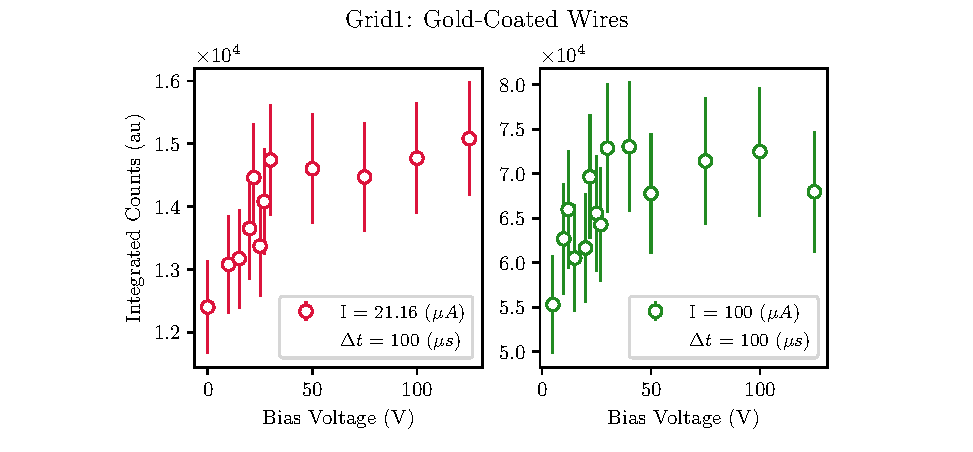
\includegraphics[width=\columnwidth]{IntensityScan/Grid1_IntensityScan.pdf}
    \end{subfigure}
    \begin{subfigure}{1.0\columnwidth}
        \centering
        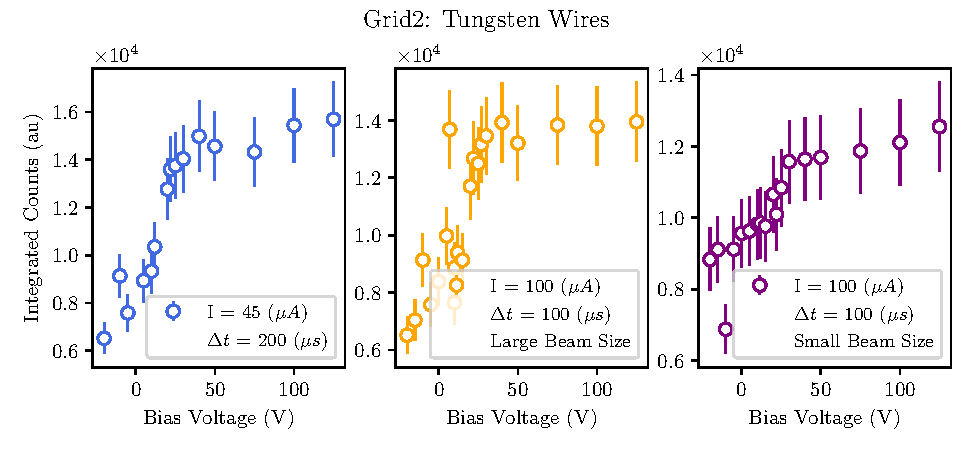
\includegraphics[width=\columnwidth]{IntensityScan/Grid2_IntensityScan.pdf}
    \end{subfigure}
    
    \caption{Integral of the signal registered by the SEM grids as a function of the applied bias voltage. Top figures: Gold-Coated Tungsten Wires. Bottom Figures: SEM grid with pure tungsten wires. }
    \label{fig:BiasScan}
\end{figure}

Figure \ref{fig:BiasScan} shows the measured integrated number of particles as a function of the bias current applied for different beam conditions. In all the different cases, we can observe how the total signal increases until reaching saturation for bias voltages above $\sim$ 40 V. For negative bias voltages the signal diminishes. This signal was also expected to saturate for negative values. However, this could not be observed during the measurements for the applied voltages. 

\subsection{Profile Measurement and Time Studies}

The effects of the bias voltage can also be observed in the measurements of the transverse beam profile. Figure \ref{fig:BeamProfileBiasEffect} shows, for different bias voltages, the transverse profile of the beam. Lighter colors indicate larger bias voltages. With these measurements, we confirm our previous statement, higher bias voltages induce an overall higher signal along the wires. Compared to the previously installed SEM grids at GSI, the SEM grids manufactured by PROACTIVE provide a much larger resolution. A comparison between the measurements taken by the GSI grid and the PROACTIVE grid is shown in Figure \ref{fig:OldNewProfCompa}. Due to the differences in the data acquisition systems, to compare these measurements normalization of the intensity and an offset correction had to be applied.
\vspace{-0.4cm}
\begin{figure}[h]
    \centering
    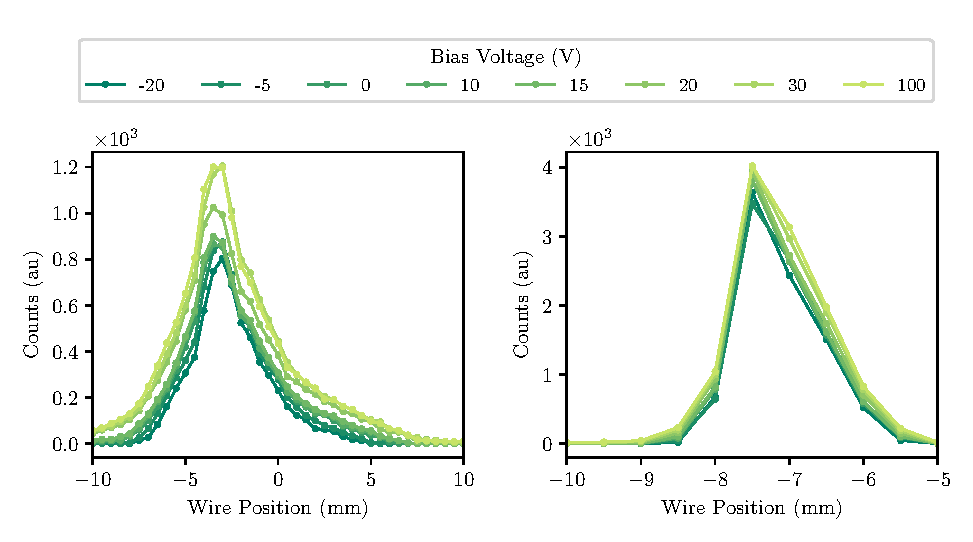
\includegraphics[width=1.0\columnwidth]{BeamProfileBiasEffect/SemGridProfileBiasCompa.pdf}
    \caption{Effect of Bias vvoltage on transverse beam profile measurements. Both profiles were measured with Grid2. Left: $\Delta t = 200 $ $\mu s$, I = 45 $\mu A$. Right:  $\Delta t = 100 $ $\mu s$, I = 100 $\mu A$ . }
    \label{fig:BeamProfileBiasEffect}
\end{figure}

In the case of the PROACTIVE grid, the POLAND+CSA electronics \parencite[]{ref:ElectronicsSEMgsi} allowed for measurements of the transverse beam profile as a function of time. The time resolution could be varied between 100 ns and 86 s per time slice. For these measurements, a time resolution of 5 $\mu s$ per time slice was used. Figure \ref{fig:FancyTime1} shows a measurement of the beam profile as a function of time. This measurement was taken with Grid1, with an applied bias voltage of 100 V. In this figure, one can observe that the signal registered by each wire increases during the beam passage, it reaches a maximum at the end of the beam pulse. This effect is more clear when looking at the projection of Figure \ref{fig:FancyTime1}  onto the time axis. This projection is shown in figure \ref{fig:TimeDepProje} along with the projections for two other beam conditions. 

\begin{figure}[h]
    \centering
    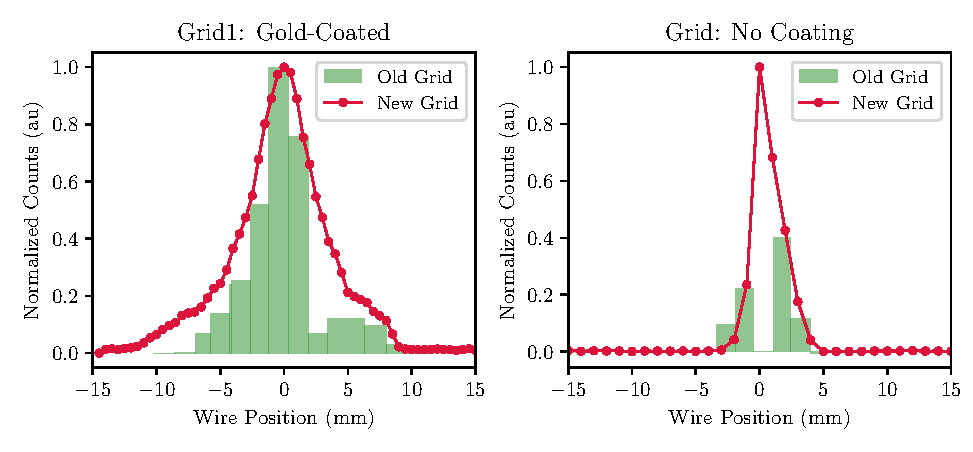
\includegraphics[width=1.0\columnwidth]{OldNewProfileCompa/OldNewProfileCompa.pdf}
    \caption{Comparison of transverse beam profile measured by GSI grid and PROACCTIVE Grid. In both cases, $\Delta t = 100 $ $\mu s$ and I = 100 $\mu A$. A bias voltage of 40 V was applied to the PROACTIVE grids.}
    \label{fig:OldNewProfCompa}
\end{figure}


Figure \ref{fig:TimeDepProje} shows the total number of counts, registered by the wires as a function of time. In this how the three signals increase until reaching a maximum and then decrease exponentially. The maximum of the curves gives us information on the beam pulse length. The time dependency of the 100 $\mu s$ and 200 $\mu s$ particle beam, shows a very clear agreement. The signal for the 100 $\mu s$ particle beam shows a very linear increase whereas the 200 $\mu s$ shows a slight logarithmical increase. This could suggest a possible signal saturation in the latter case. The big discrepancies on the 40 $\mu s$ curve suggest that a different time slice resolution was used. However, no record of that number was available in the stored data. 


\begin{figure}[h]
    \centering
    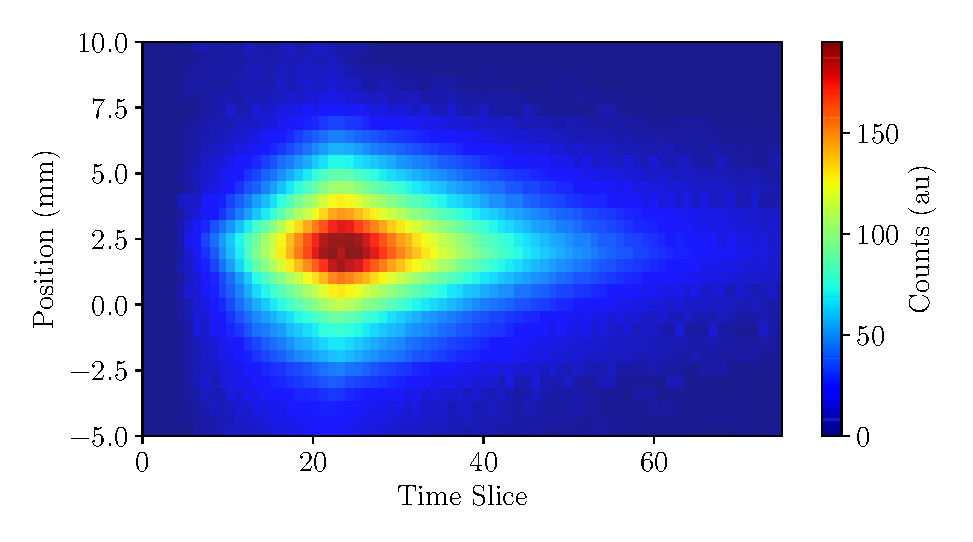
\includegraphics[width=0.9\columnwidth]{FancyProfileWithTime/FancyTimeEvolution.pdf}
    \caption{Time dependent transverse beam profile. Each time slice has a record of 5 $\mu s$. The beam pulse length and intensity were $\Delta t = 100 $ $\mu s$.}
    \label{fig:FancyTime1}
\end{figure}


By default, the transverse beam profile was calculated using the total integral of the signal over time. However, one can also study the intra-pulse transverse beam profile evolution. To illustrate this we use a measurement taken by Grid 2, for a beam of I = 100 mA and $\Delta t$ = 100 $\mu s$. Figure \ref{fig:SigmaEvolutionTime} (Top) shows the transverse beam profile measured at different instants of time. The highest intensity profile is registered at slice 22, which corresponded to the ending point of the beam pulse. The red curve shows the total integral of the signal as a function of time. For visualization purposes, this curve has been reduced by a factor 8.

\begin{figure}[h]
    \vspace{-0.2cm}
    \centering
    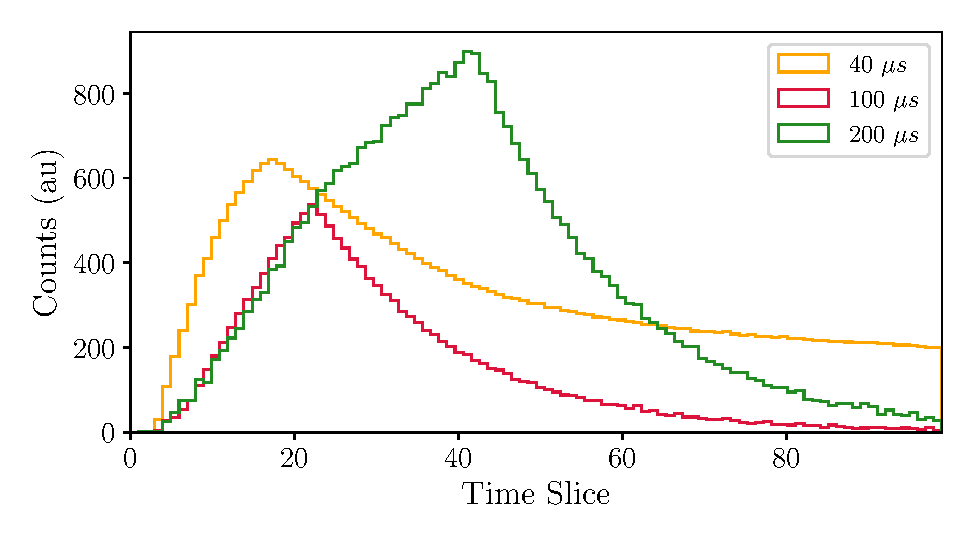
\includegraphics[width=0.8\columnwidth]{TimeEvolProj/TimeEvolutionProj.pdf}
    \caption{Integral of the total number of counts measured by all the grid wires as a function of time. For three different beam conditions. Measured with Grid1, bias voltage 100 V. }
    \label{fig:TimeDepProje}
\end{figure}
\vspace{-0.5cm}
\begin{figure}[h!]
    \centering
    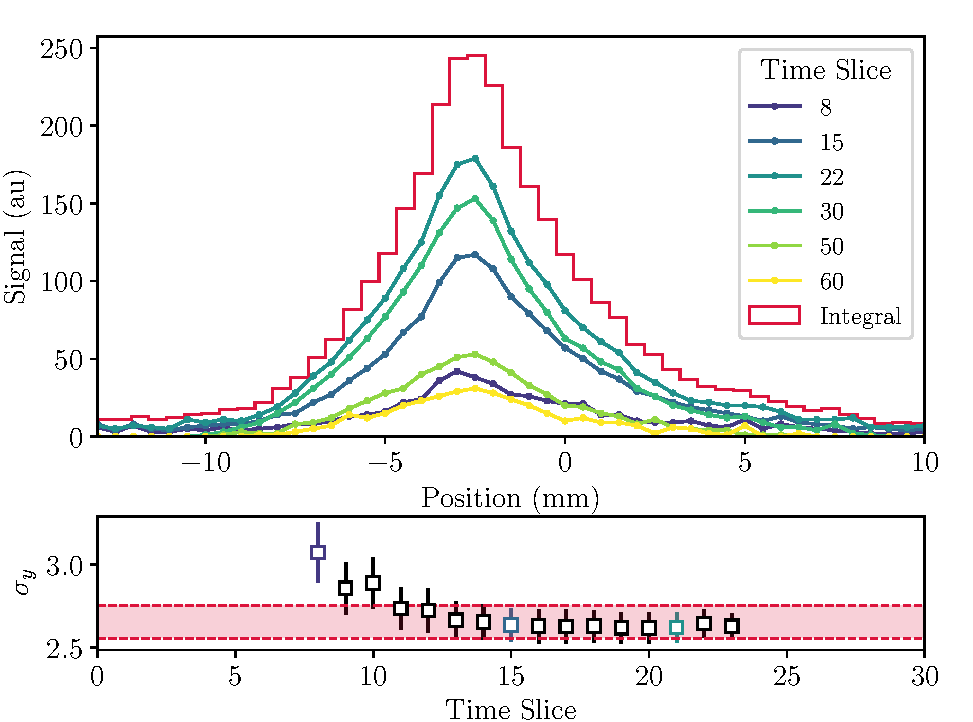
\includegraphics[width=0.8\columnwidth]{BeamProfileWithTime/BeamSigmaWithTime.pdf}
    \caption{Top: Transverse beam profile at different instants of time. Each color represents a time slice. Each time slice has a record of 5 $\mu s$. In red the total integral of the counts along the time is represented. Bottom: Vertical beam size as a function of time. Calculated by gaussian approximation of the beam to each time slice. In red, $\sigma_y$ of the beam is calculated in the integral beam profile. }
    \label{fig:SigmaEvolutionTime}
\end{figure}

If one assumes a gaussian approximation, the $\sigma$ of the beam can be obtained. Figure \ref{fig:SigmaEvolutionTime} (bottom) shows the evolution of the fitted $\sigma$ to the experimental data as a function of time. The uncertainties in these values are solely due to the uncertainties in the parameter fitting. These results show that measured the $\sigma$ of the beam is larger at an earlier time and then it stabilizes. This could be due to real intra-pulse beam size differences or simply because the registered signal is not strong enough for doing a proper Gaussian fitting. The fitted $\sigma$ for the integral measurement (represented as a red stripe) matches very well the calculated values of the $\sigma$ at the core of the beam pulse. 

\subsection{Thermal Studies}

To prove the suitability of the SEM grids to the demanding conditions of the future pLinac, a systematic set of measurements was performed. Both grid prototypes were irradiated in the regular UNILAC 'grid protection mode', with a beam intensity of $I = 500 \mu A $ and a beam pulse length of $40 \mu s$. From this safe condition, the intensity of the beam was gradually increased while measurements of the beam profile were taken. In parallel to the measurements, simulations for wire heating were done with the pyTT code, predicting the wire temperature at the various beam conditions. 

It is important to remember that the pyTT code is currently optimized for thin target detector measurements. This means the range of the incident particles is much larger than the thickness of the material, so the beam only deposits a small part of its energy in the detector and this energy deposition is constant along the detector length. In this case, the wires are thick compared to the range of 8.6 MeV/u Argon ions in tungsten (Wire thickness = 100 $\mu m$, particle range = 11.9 $\mu m$). This has two major consequences: 

\begin{itemize}
    \item We need to find an equivalent energy deposition as the program will consider a constant energy deposition along the detector. For these simulations, two extreme cases were considered. The energy deposition can be overestimated assuming the maximum energy is deposited along the whole length, or it can be underestimated assuming the maximum energy is spread along the whole length. The real value will lie in between this two. A more in-depth study should be performed if a more accurate value is needed. 
    \item An extra contribution of conduction cooling is possible along the beam direction. This might make the simulated cooling slower than the real one. In reality, the thermal equilibrium might be reached earlier than predicted in the simulations. 
\end{itemize}

\subsubsection{Grid 1, Gold-Coated Tungsten Wires}

An initial assessment of the beam size was performed with the upstream SEM grid, this measurement is shown in Figure \ref{fig:BeamProfileStudy1}. A gaussian approximation of the beam yielded a beam size of $\sigma_x = 3.19(26)$ mm and $\sigma_y = 1.694(16)$ mm. In this case, we can observe a big difference between the maximum intensity registered by the horizontal ($\sim$ 3.80 au) and the vertical ($\sim$ 12.86 au) measurements. The particle distribution in the horizontal plane seemed to be more planar than gaussian. This might suggest that the density of particles in the horizontal plane was not as high as the one in the vertical plane. 

\begin{figure}[h]
    \centering
    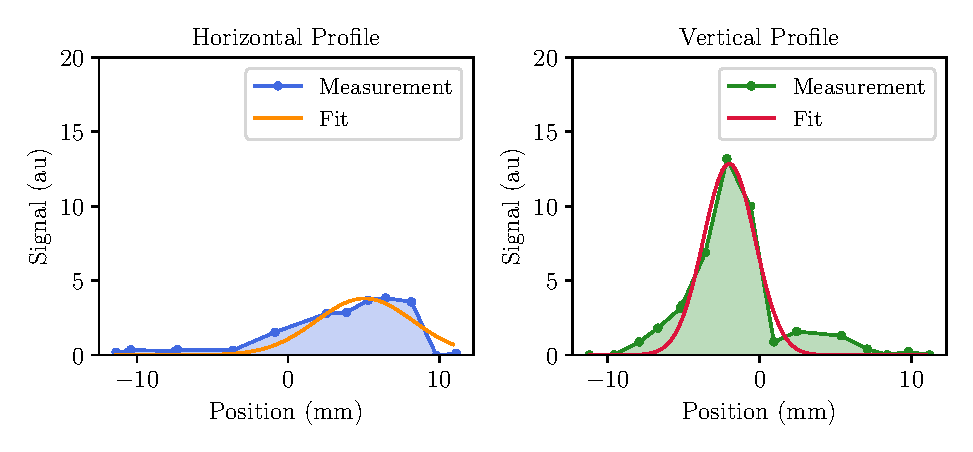
\includegraphics[width=1.0\columnwidth]{ThermalStudyBeamProfile1/ProfileMeasurementStudy1.pdf}
    \caption{Beam profile measured with GSI SEM grid with, Gaussian fit for beam size determination.}
    \label{fig:BeamProfileStudy1}
\end{figure}

The beam pulse length was kept constant at 40 $\mu s$, with a repetition rate of 1 Hz. The beam intensity was gradually increased, from 0.5 - 1.5 mA. Figure \ref{fig:MaxTempStudy1} (left) shows the simulated temperature evolution of the detector as a function of time. For three of these beam intensities. The figure on the right shows in more detail the predicted maximum temperature for the different beam intensities. The big uncertainties in the simulated results come from the uncertainties in the energy deposition in the detector material.

\begin{figure}[h]
    \centering
    \includegraphics[width=1.0\columnwidth]{Study1MaximumTempSim/MaximumTempSim1.pdf}
    \caption{Left Plots: Evolution of the maximum temperature reached by a gold-coated tungsten wire for 5 beam shots. Right: Maximum temperature reached for different beam intensities. }
    \label{fig:MaxTempStudy1}
\end{figure}

These results predicted that the wire would be able to sustain all the applied beam intensities, although beam intensities larger than 1.5 mA approach dangerous territory. The melting point of gold is $\sim$ 1400K. From the simulation results, we concluded that, for beam intensities $\geq$ 0.6 mA, the gold should have evaporated from the surface. 

The beam profile was measured for four different beam intensities. The results of these measurements are shown in figure \ref{fig:FancyStudy1Plot}. Grid1 was able to measure the beam profile for all the given beam intensities without any problem. There are also no visual effects of wire heating (thermionic emission) or wire damage in the measurements. Indeed, after the measurements were performed the grid was extracted from the accelerator for a visual inspection. The SEM grid was intact, including the gold coating in the central wires. 

This proves that the simulations were overestimating the beam heating in the wire. This overestimation might come from two factors: the gaussian approximation of the horizontal beam profile. And an overestimation in the energy deposition along the wire length.  

\begin{figure}[h]
    \vspace{-0.4cm}
    \hspace{0.1cm}
    \centering
    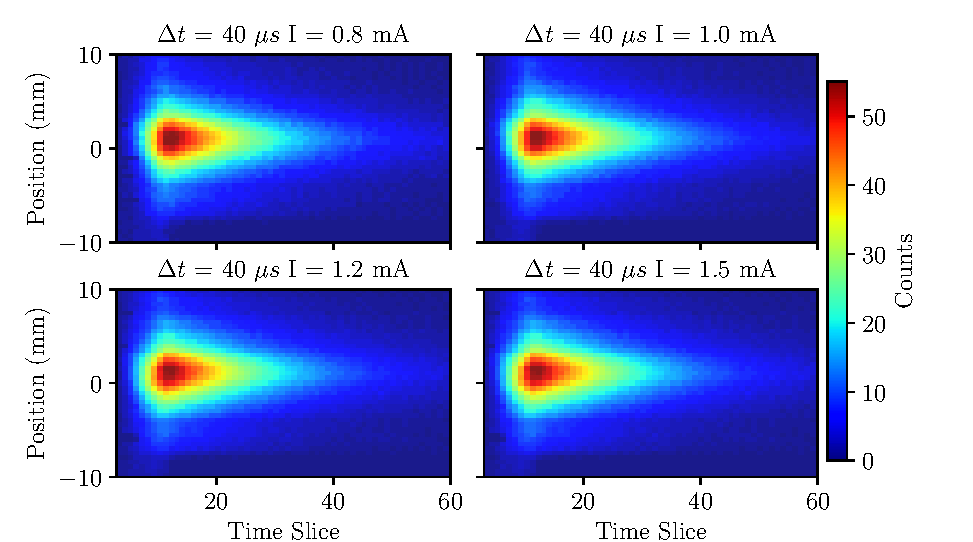
\includegraphics[width=1.0\columnwidth]{FancyPlotStudy1/FancyMeasStudy1.pdf}
    \caption{Signal measured by the different wires as a function of time. For four different beam intensities. }
    \label{fig:FancyStudy1Plot}
\end{figure}

\subsubsection{Grid 2, Pure Tungsten Wires}

For testing the second grid, we made sure that Gaussian approximation of the beam was accurate for both the horizontal and the vertical planes. Figure \ref{fig:BeamProfileStudy2} shows the beam profile measured with the GSI grid for this second set of measurements. In this case, $\sigma_x = 2.052(37)$ mm and $\sigma_y = 1.587(91)$ mm. The beam pulse length was also 40 $\mu s$ and the repetition rate was 1 Hz. The beam intensity varied form 0.5 - 1.5 mA. 

The maximum temperature evolution as a function of time for different intensities is shown in Figure \ref{fig:MaxTempStudy2}. Due to the smaller beam size, the maximum predicted temperatures are larger than the ones predicted in the previous case. If the overestimation of the energy deposition is considered, the simulation predicted a wire breakage for beam intensities $\geq$ 0.6 mA. Even in the average case, the simulations predicted the wire would break in the case of 1.5 mA beam intensity.

\begin{figure}[h]
    \centering
    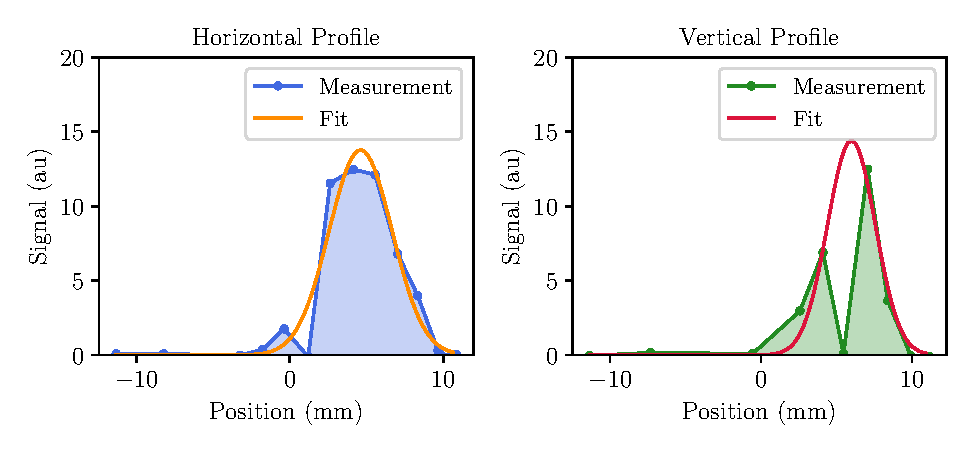
\includegraphics[width=1.0\columnwidth]{BeamSizeStudy2/BeamProfileMeasurement2.pdf}
    \caption{BeamProfile measured with GSI SEM grid for the second study with Gaussian fit for beam size determination.}
    \label{fig:BeamProfileStudy2}
\end{figure}

Figure \ref{fig:FancyStudy2Plot} shows the experimental measurements of the beam profile for the different intensities. For a beam pulse length of 40 $\mu s$ the grid seemed to resist the beam load very well,  even for a 1.5 mA beam current. The simulations are again overestimating the wire's maximum temperature. Because we really wanted to cross-check the power limit of the grid we went one step further and increased the beam pulse length to up 70 $\mu s$. This increases the number of particles reaching the detector by a factor 1.7 (comparing it to the $\Delta t$ = 40 $\mu s$ case). 

Figure \ref{fig:FancyStudy2Plot} also shows the results of the measurements taken for this longer pulse, for three different instants of time. First, we can observe a wire current that extends much longer than the beam pulse length. This was followed by a wire breakage, which in this figure is represented by the lack of signal in the wire.  A visual exploration of the grid after the experiment confirmed the wire was broken.


\begin{figure}[htb]
    \centering
    \includegraphics[width=1.0\columnwidth]{Study2MaximumTempSim/MaximumTempSim2.pdf}
    \caption{Left Plots: Evolution of the maximum temperature reached by a pure tungsten wire for 5 beam shots. Right: Maximum temperature reached for different beam intensities. }
    \label{fig:MaxTempStudy2}
\end{figure}


\begin{figure}[htb]
    \centering
    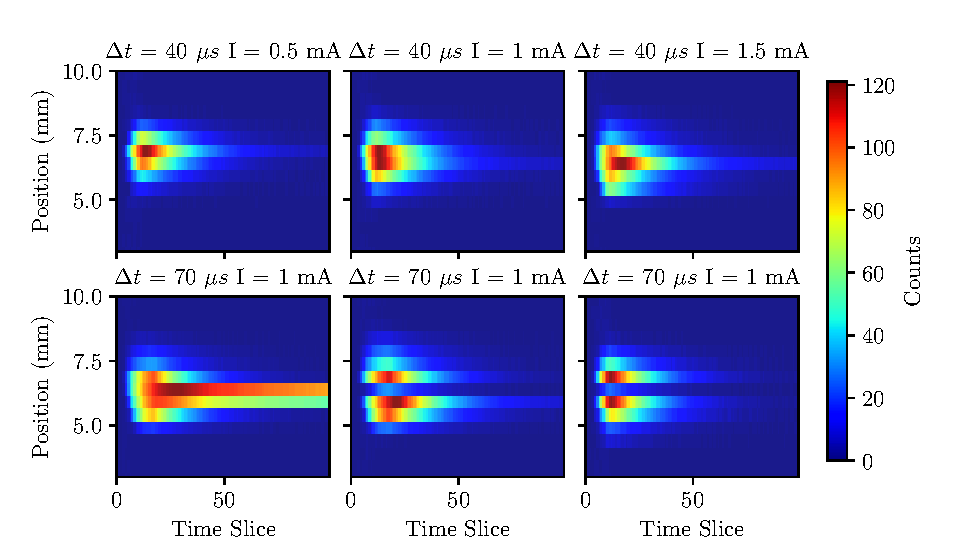
\includegraphics[width=1.0\columnwidth]{FancyPlotStudy2/FancyFigurePlot.pdf}
    \caption{Fancy beam profile as time measurement for study 2}
    \label{fig:FancyStudy2Plot}
\end{figure}


Figure \ref{fig:ProjectionOfStudy2} shows a projection of the current, registered by different wires, as a function of time. When the beam pulse length was  $\Delta t$ = 40 $\mu s$, the expected time distribution is observed. The signal increases until the end of the beam pulse and then it decreases exponentially. For a $\Delta t$ = 70 $\mu s$, the two wires that were measuring the central part of the beam show a different time distribution. The signal increases until the end of the beam but it does not decrease exponentially. This could be explained by the presence of thermionic emission electrons. This thermionic electrons, because they are negative charges leaving the detector material, could affect the registered current, making it larger than it should for a small period of time. 

The analysis performed at LINAC4 to obtain the temperature from the thermionic current measurement (Shown in Chapter \ref{ch:ThermoMeas}, Section \ref{sec:ThermoMeas}) could not be performed for these measurements. In this case, it is not straightforward to disentwine the current generated from thermionic emission from the one coming from the capacitive discharge.  

\begin{figure}[htb]
    \centering
    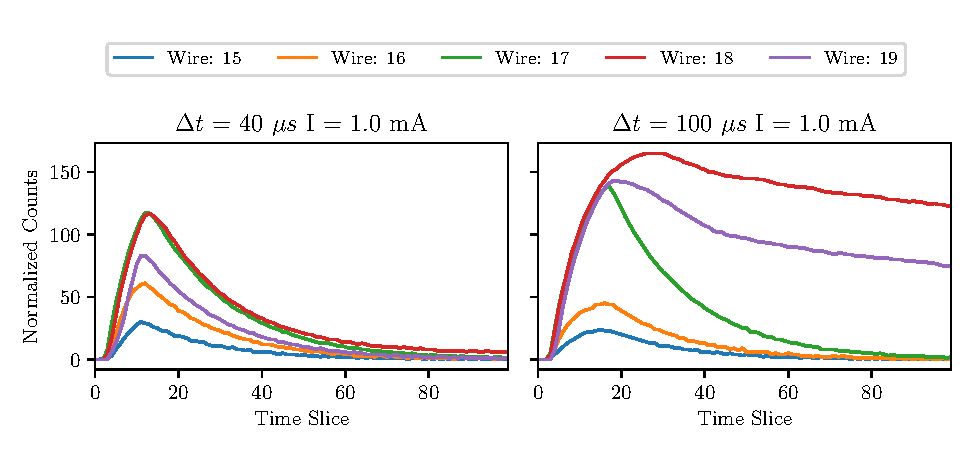
\includegraphics[width=1.0\columnwidth]{TimeEvolutionProjStudy2/TimeEvolutionStudy2.pdf}
    \caption{Current registered by the different wires in the pure tungsten grid as a function of time. For two different beam pulse lengths. }
    \label{fig:ProjectionOfStudy2}
\end{figure}
